\section{Reproducing the experiments with numerical models} \label{sec:exp_vs_num}
As outlined in Section~\ref{sec:introduction}, the purpose of this section is to discuss the relevance of three specific points concerning the hydrodynamic modeling in the numerical simulations, in light of the experimental results: the drag forces on the pontoons (Section~\ref{subsec:exp_vs_num:drag}); the need for second-order wave forces not only for the horizontal motions, but also for the vertical dofs (Section~\ref{subsec:exp_vs_num:2nd_order}); and whether the mean hull inclination induced by the wind needs to be considered in the solution of the radiation/diffraction problem (Section~\ref{subsec:exp_vs_num:impact_inclination}). After these aspects have been discussed, Section~\ref{subsec:exp_vs_num:main_results} summarizes the main results to show the adherence between the numerical simulations and the experiment.


\subsection{The need for drag forces on the pontoons} \label{subsec:exp_vs_num:drag}
The first point concerns the drag forces on the pontoons of the hull, which are relevant not only due to the damping that they introduce, but also because drag is and important forcing term for this type of floater. These forces are modeled in OpenFAST using Morison elements, but since the current version of the software includes only circular elements, the source code was modified to account for elements with rectangular cross section. In this modified version, the drag forces per unit length are given by:
\begin{equation}
\begin{split}
	f_{Dx} &= \frac{1}{2} \rho \mkern2mu C_{Dx} \mkern2mu D_x \,||\vec{u}|| \, u_x \\[6pt]
	f_{Dy} &= \frac{1}{2} \rho \mkern2mu C_{Dy} \mkern2mu D_y \,||\vec{u}|| \, u_y
\end{split}		
\end{equation}
%
where $\vec{u}=u_x\vec{e}_1+u_y\vec{e}_2$ is the relative fluid velocity (i.e. the difference between fluid velocity and local body velocity); $\vec{e}_1$ and $\vec{e}_2$ are the unit vectors directed along the local $x$ and $y$ axes, which are normal to the lateral faces of the rectangular cylinder; $C_{Dx}$ and $C_{Dy}$ are the drag coefficients in each direction; and $D_x$ and $D_y$ are the sides of the rectangle.

The drag coefficients in each direction are obtained by matching numerical decays in surge and heave with their experimental counterparts, as illustrated in Figures~\ref{fig:exp_vs_num:drag:surge_decay}~and~\ref{fig:exp_vs_num:drag:heave_decay}. These decays were performed with the complete setup of the experiment, hence with both the mooring lines and the umbilical cables needed by the SIL method, but without either wind or waves. On the right side of each graph is presented a PQ-analysis~\citep{burmester2020}, in which the slope of the curve corresponds to the quadratic damping, while the intersection with the $y$ axis is proportional to the linear damping. It turns out that the latter, which is mostly due to wave radiation, is negligible, being relevant only when the amplitude of motion is very small (note that the experiment provides a negative value for the linear heave damping, which is clearly not physical and a consequence of the small values involved). On the other hand, the quadratic damping, which is obtained considering the drag coefficients summarized in Table~\ref{tab:exp_vs_num:drag:drag_coeffs}, is within the range measured in the experiments (3 repetitions in surge and 7 in heave), as shown by the values presented in the same figures (a complete set of decay results is given in Table~\textcolor{red}{5}). Note that it would be impossible to match the damping levels in both dofs simultaneously if the pontoons were modeled using circular Morison elements, since both $D$ and $C_D$ are different for each direction. 
\begin{figure*}[!hbtp]
	\centering
	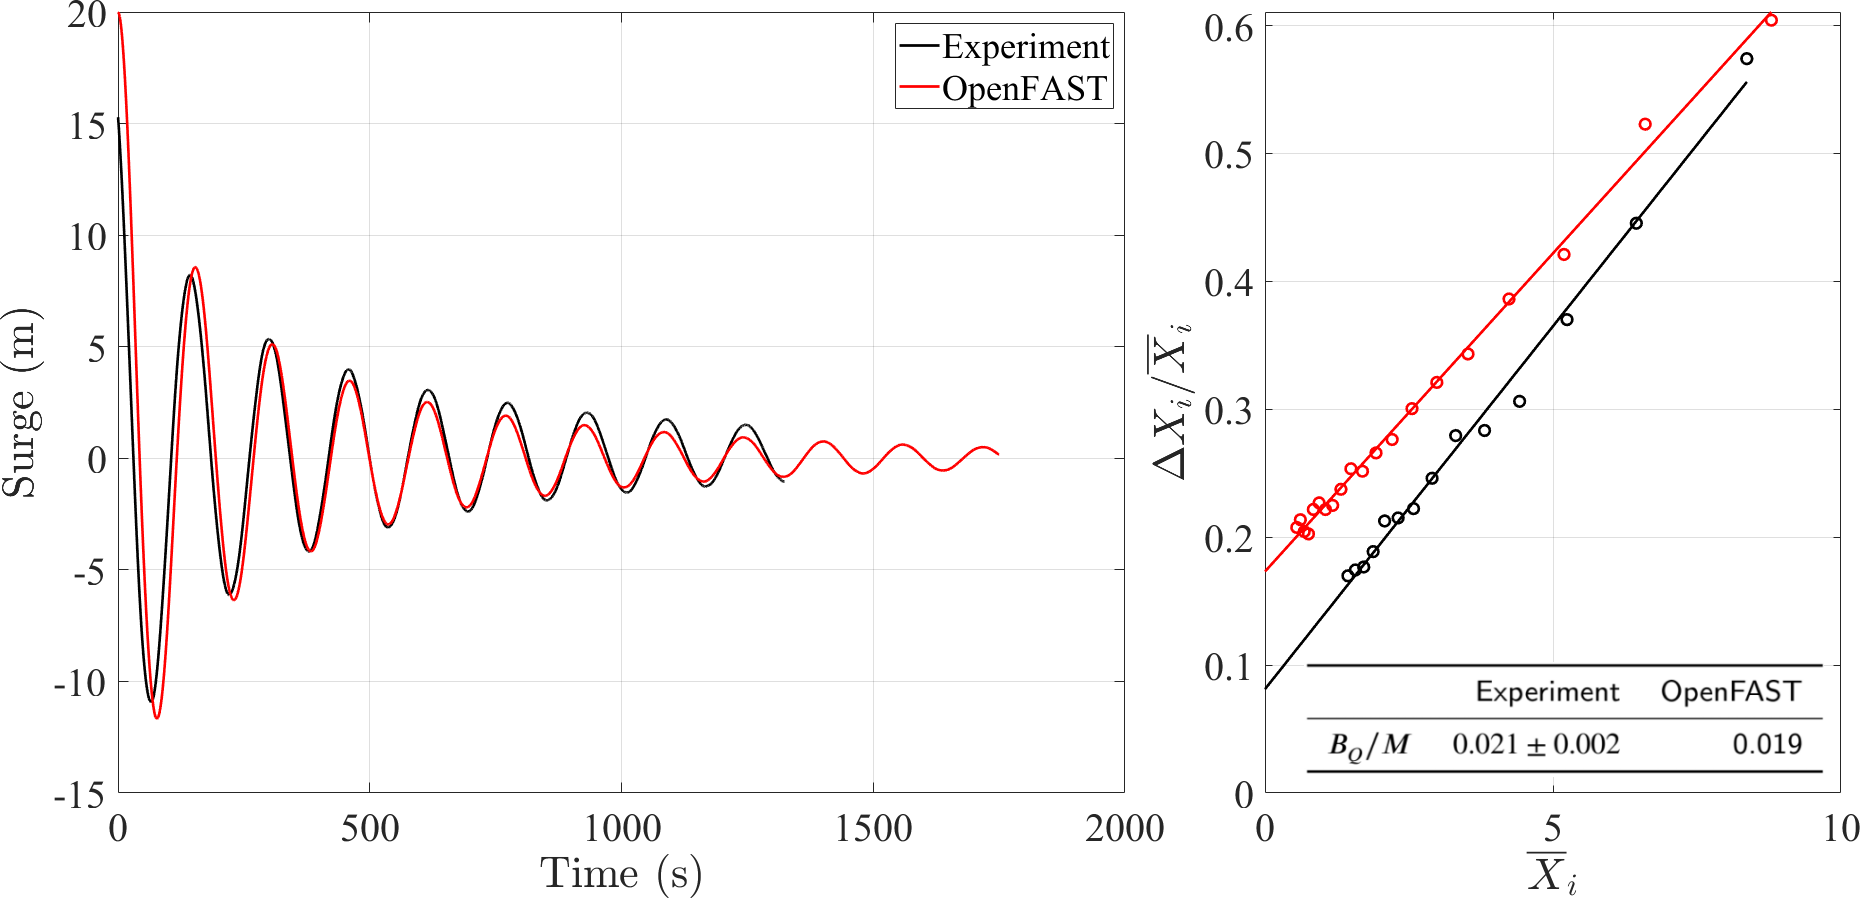
\includegraphics[width=0.80\textwidth]{./figures/surge_decay_drag_pontoon.png}%	
	\caption{Comparison of numerical and experimental surge decays. $B_Q/M$ is the nondimensional quadratic drag coefficient.} \label{fig:exp_vs_num:drag:surge_decay}%
\end{figure*}%

\begin{figure*}[!hbtp]
	\centering
	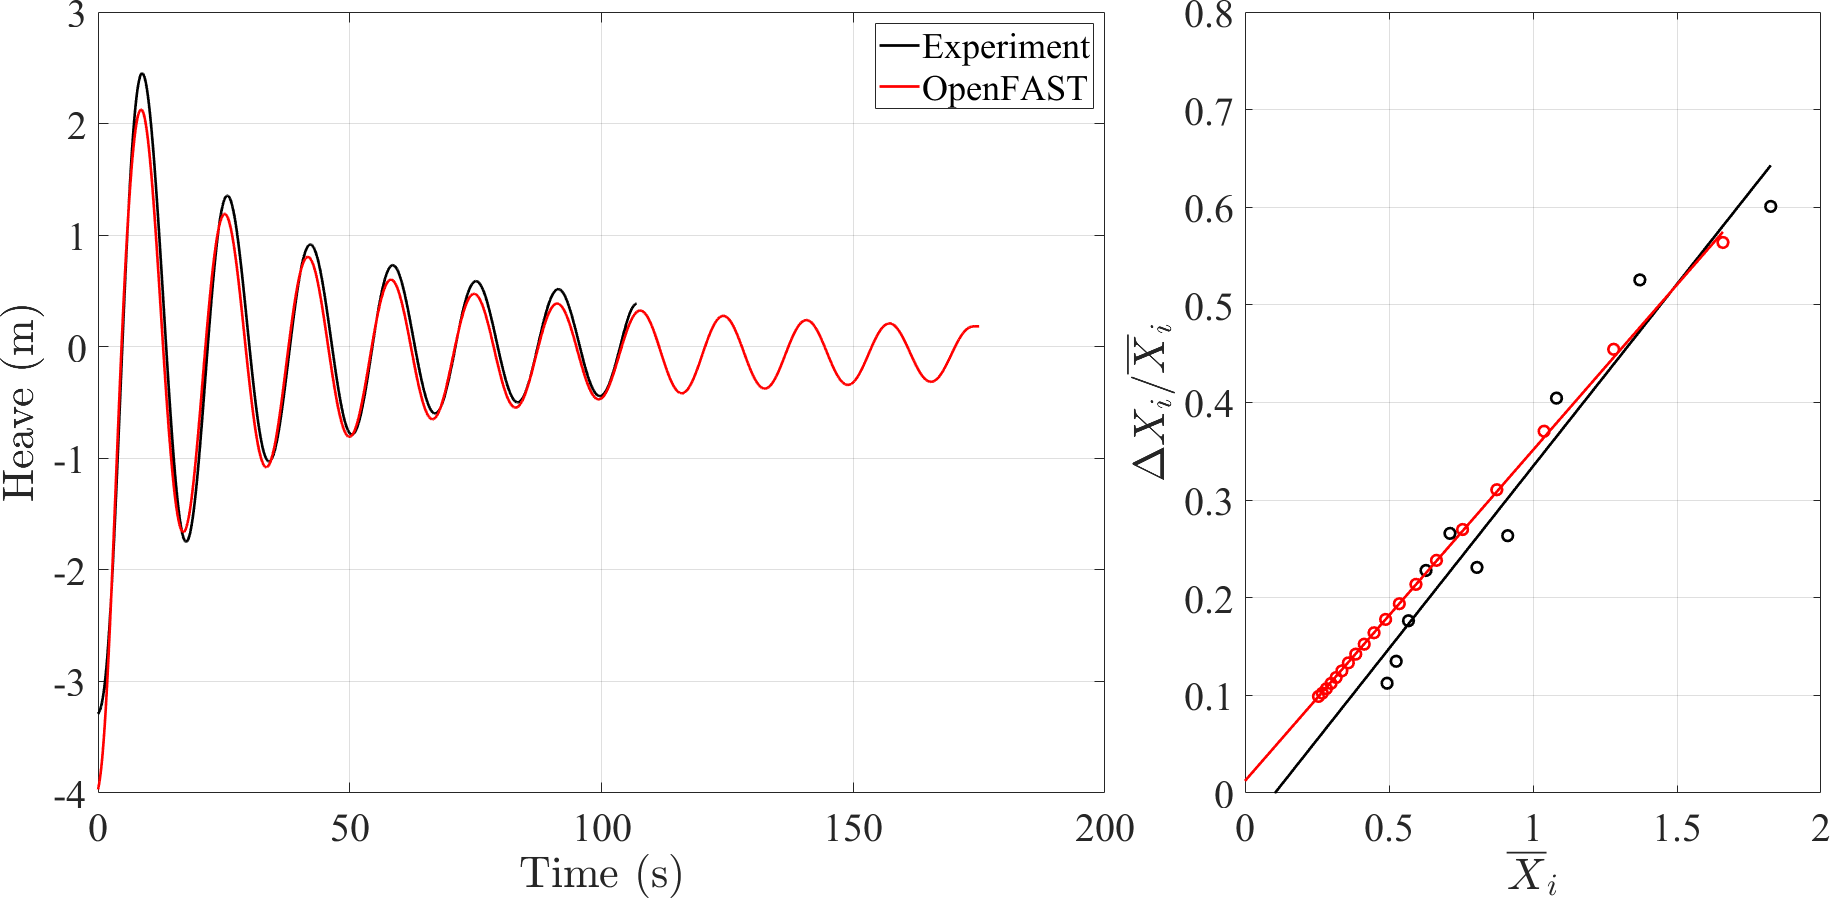
\includegraphics[width=0.80\textwidth]{./figures/heave_decay_drag_pontoon.png}%	
	\caption{Comparison of numerical and experimental heave decays. $B_Q/M$ is the nondimensional quadratic drag coefficient.} \label{fig:exp_vs_num:drag:heave_decay}%
\end{figure*}%

Though the drag coefficients obtained from decay tests are not necessarily the same required by simulations considering waves, the values provided in Table~\ref{tab:exp_vs_num:drag:drag_coeffs} have led to good results for all the wave and wind conditions analyzed in this work, as will be shown in Section~\ref{subsec:exp_vs_num:main_results}. For now, a single test case is enough to illustrate the influence of the drag forces. For that, Figures~\ref{fig:exp_vs_num:drag:ptfmsurge}~and~\ref{fig:exp_vs_num:drag:ptfmheave} present the surge and heave motions of the FOWT under the action of the IRR-I1 wave ($T_P=14.5\,\text{m}$ and $H_S=9.3\,\text{m}$) and an incidence of -10\textdegree{}, without wind effects. To evidence the importance of the drag forces, the plots include results of simulations performed with circular Morison elements calibrated for the opposite dof, i.e. the results labeled \enquote{OpenFAST - Circ. S} presented in the heave graphs correspond to a circular pontoon with $D=6.0\,\text{m}$ and $C_D=2.50$, which are the values obtained from the surge decays; conversely, \enquote{OpenFAST - Circ. H} correspond to a circular pontoon calibrated using the heave decays.
\begin{table}[!hbtp]
	\caption{Resulting drag coefficient for each Morison element and its main dimensions.}\label{tab:exp_vs_num:drag:drag_coeffs}
	\begin{tabular}{lrrr}
		\toprule
		& Length & Diameter & $C_D$ \\
		\midrule
		Central column & 18.6 & 14.1 & 0.61 \\
		Offset columns & 18.6 & 17.0 & 0.61 \\
		Pontoons - Vertical & 23.0 & 17.0 & 12.00 \\
		Pontoons - Horizontal & 23.0 & 6.0 & 2.50 \\
		\bottomrule%
\end{tabular}%
\end{table}%

The first set of graphs, Figure~\ref{fig:exp_vs_num:drag:ptfmsurge}, shows that the difference in drag models has a significant impact on the surge motion only around its resonance frequency, which is expected due to the different damping levels. However, the slow surge motion is underpredicted even by the OpenFAST model with rectangular pontoons and drag coefficients calibrated from decay tests. The main hypothesis is that this is related to an underprediction of the low-frequency force rather than an overprediction of damping, following the findings by \citet{wang2022oc6}, who showed that a third-order force that arises from computing the drag loads considering the instantaneous wave elevation (as opposed to the approach considered in this work, which integrates drag loads up to the mean water level) explained the underprediction of the slow surge motion reported by \cite{OC52017}. 

The impact of drag on heave is more critical than observed for surge, as illustrated in Figure~\ref{fig:exp_vs_num:drag:ptfmheave}. In this case, it acts not only by damping the resonant response around $16.5\,\text{s}$ ($0.061\,\text{Hz}$), but also as a relevant forcing term around $15\,\text{s}$ ($0.067\,\text{Hz}$). This is made clear by the Heave RAOs plotted on the bottom right of the same figure, which show that the response predicted by WAMIT is almost zero at $15\,\text{s}$, a consequence of the force obtained with potential flow being null close to that period, while the result with OpenFAST considering the rectangular pontoon adheres very well to the experiment. This means that it would not be possible to model this behavior by tuning an external quadratic damping coefficient, as neglecting this forcing term would lead to important underpredictions of the motions. 

Still about heave, it is noteworthy that a single set of drag coefficients, obtained from such a simple procedure as a decay test and using an equally simple approach as Morison's equation, was able to model pretty well both the situation in which drag acts by damping the motion and the one in which it plays the role of a forcing term.
\begin{figure*}[!hbtp]
	\centering
	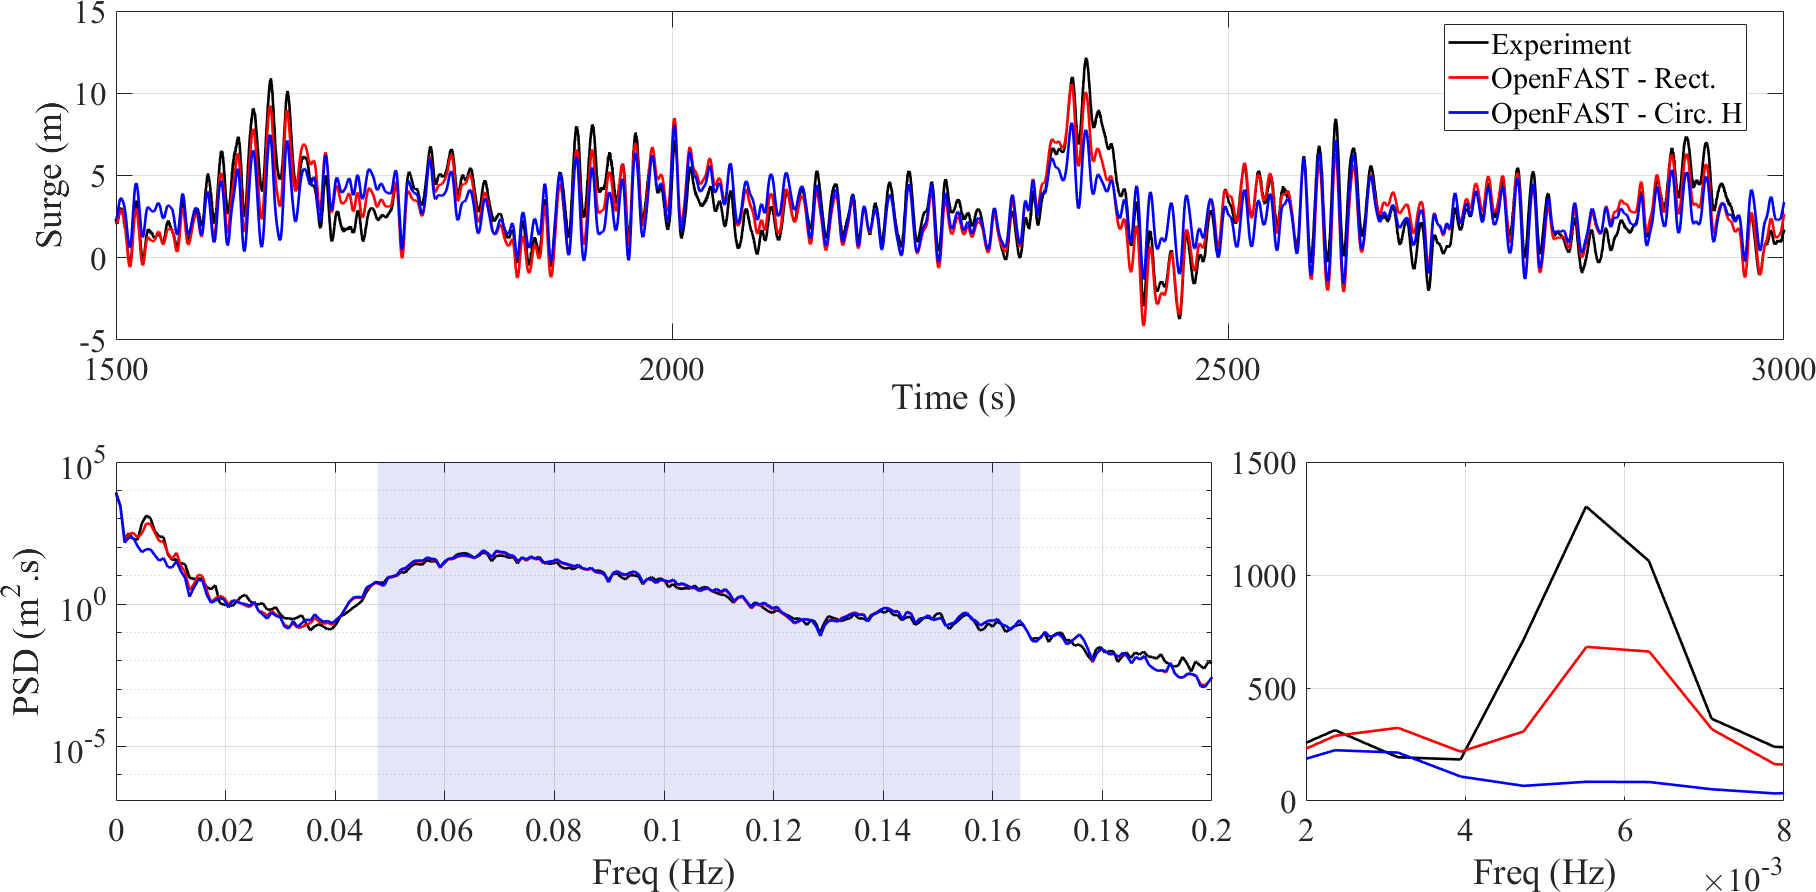
\includegraphics[width=0.9\textwidth]{./figures/ptfmsurge-drag_pontoon.png}	
	\caption{Illustration of the influence on surge motions due to drag forces on the pontoons (IRR-I1 wave, incidence of -10\textdegree{}, without wind effects). The bottom right plot is a zoom in linear scale of the PSD around the resonance frequency of surge (about $0.006\,\text{Hz}$). The range of frequencies corresponding to the incoming waves is shaded in blue.} \label{fig:exp_vs_num:drag:ptfmsurge}
\end{figure*}

\begin{figure*}[!hbtp]
	\centering
	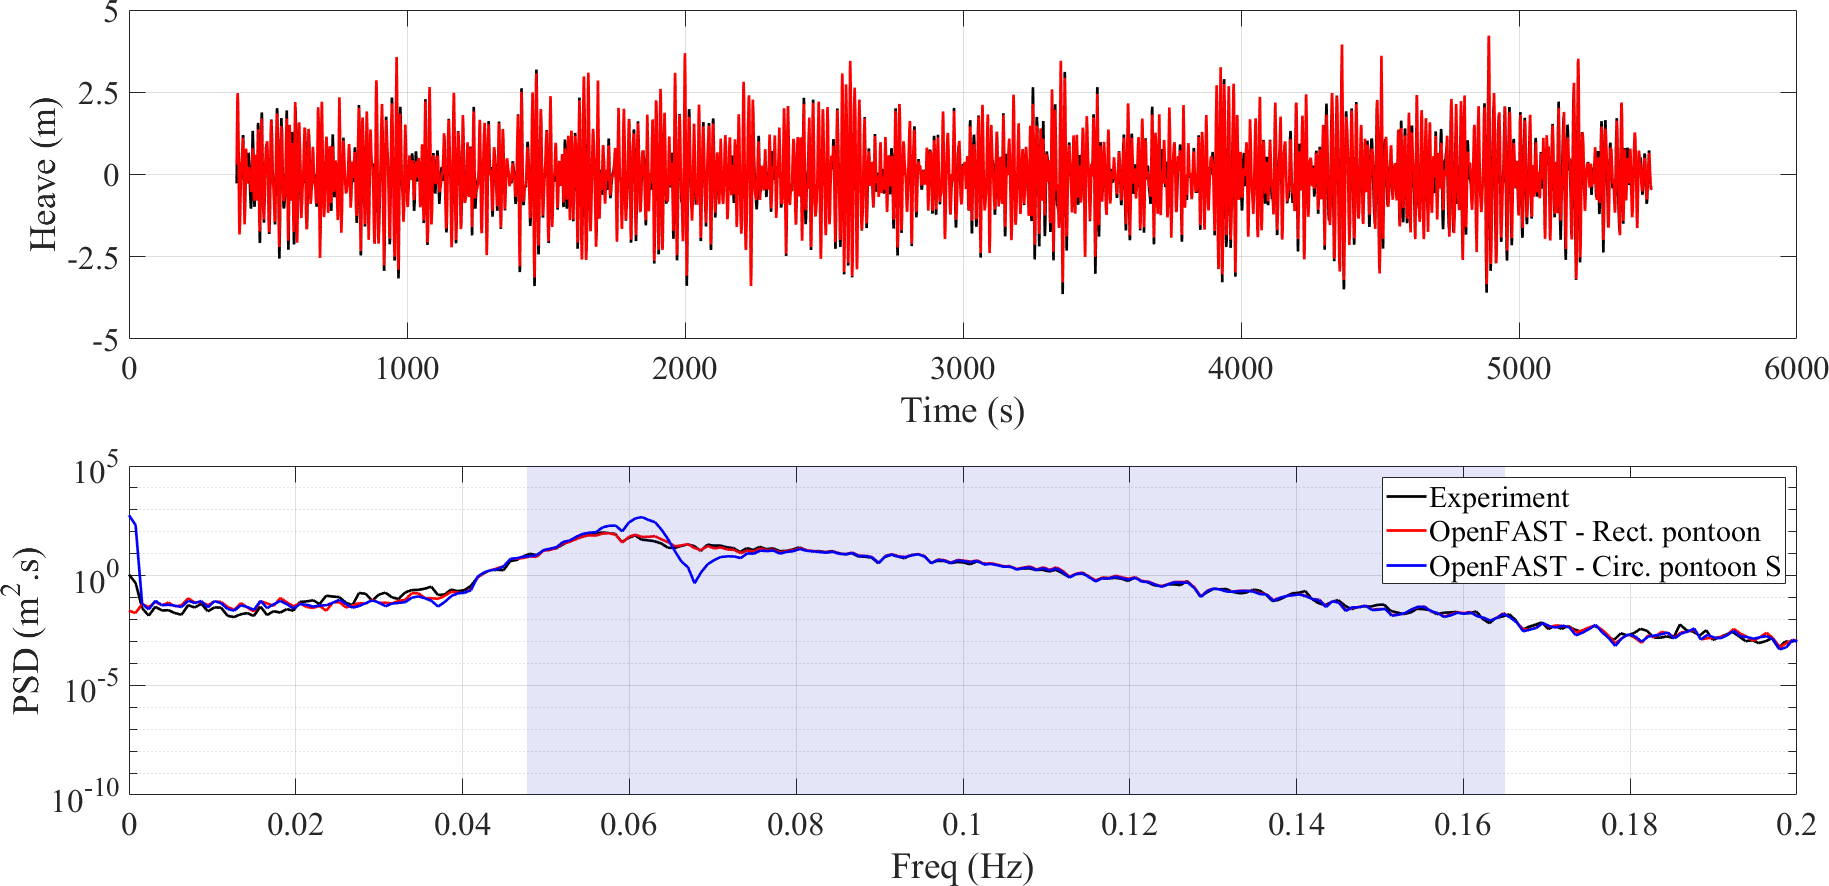
\includegraphics[width=0.9\textwidth]{./figures/ptfmheave-drag_pontoon.png}	
	\caption{Illustration of the influence on heave motions due to drag forces on the pontoons (IRR-I1 wave, incidence of 60\textdegree{}, without wind effects). The range of frequencies corresponding to the incoming waves is shaded in blue.} \label{fig:exp_vs_num:drag:ptfmheave}%
\end{figure*}%












\subsection{The importance of second-order wave forces for vertical motions} \label{subsec:exp_vs_num:2nd_order}
The relevance of low-frequency second-order wave forces on the dynamics of FOWTs is well known and documented in the literature \citep{coulling2013, gueydon2014, lopez2015, OC52017, simos2018slow}, and this section is an addition to this ongoing discussion in order to emphasize the importance of this force component not only for the horizontal motions of the floater, but also for the vertical degrees of freedom.

There are a number of approaches and simplifications that can be adopted to compute second-order forces. Due to its simplicity, the first procedure that was tested in this study was to compute the slow-drift forces using Newman's approximation \citep{newman1974}, but for the horizontal degrees of freedom only. This is a very simple approach because it only requires the mean forces/moments, which do not depend on the solution of the second-order problem, and the integrations are performed based on conservation of momentum, which is far less strict in terms of mesh convergence. For the reader familiar with WAMIT, this corresponds to the .8 files.

This approach is usually enough for the analysis of floating systems in deep waters and for which surge, sway and yaw (typically with low natural frequencies) are the only degrees of freedom that present significant slow motions. Unfortunately, this is not the case for most FOWTs, including the one analyzed in this study, and analyzes considering complete sets of QTF (Quadratic Transfer Function) matrices are required. However, as one of the objectives of this work is to analyze the impact of mean hull inclination on the solution of the radiation/diffraction problem (discussed ahead in Section~\ref{subsec:exp_vs_num:impact_inclination}), it would be unfeasible to compute the completes QTFs for all the different conditions. For this reason, an intermediate approach is adopted in which Newman's approximation is used with a mixed mean drift file in which the horizontal degrees of freedom (surge, sway and yaw) are computed with conservation of momentum (WAMIT .8 file) while the vertical motions (heave, roll and pitch) are calculated using pressure integration (WAMIT .9 file). The advantage is that the convergence of pressure integration is more complicated for the horizontal dofs than for the vertical dofs due to the larger gradient near the free-surface, so this mixed procedure saves computational time.

The results obtained for the pitch motion with each of these approaches are illustrated in Figure~\textcolor{red}{8}\footnote{The importance of slow surge forces was already made clear in Section~\ref{subsec:exp_vs_num:drag} by the resonant motion presented in Figure~\ref{fig:exp_vs_num:drag:ptfmsurge}}, considering the same wave as the previous section (IRR-I1 wave, i.e. $T_P=14.5\,\text{m}$, $H_S=9.3\,\text{m}$ and an incidence of -10\textdegree{}). It is clear that neglecting the slow-pitch forces (the simulations considering the .8 file alone) leads to an important underprediction of pitch motion: the predicted maximum angle of \textcolor{red}{2.0\textdegree{}} is considerably lower than the value of \textcolor{red}{4.0\textdegree{}} measured in the experiments. The results improve significantly when Newman's approximation is employed considering vertical mean forces (mixed .8 and .9 file), with the simulations providing a maximum angle of \textcolor{red}{4.0\textdegree{}}. MAS NO RESTANTE DO TRABALHO USEI O MISTO.

\begin{figure*}[!hbtp]
	\centering
	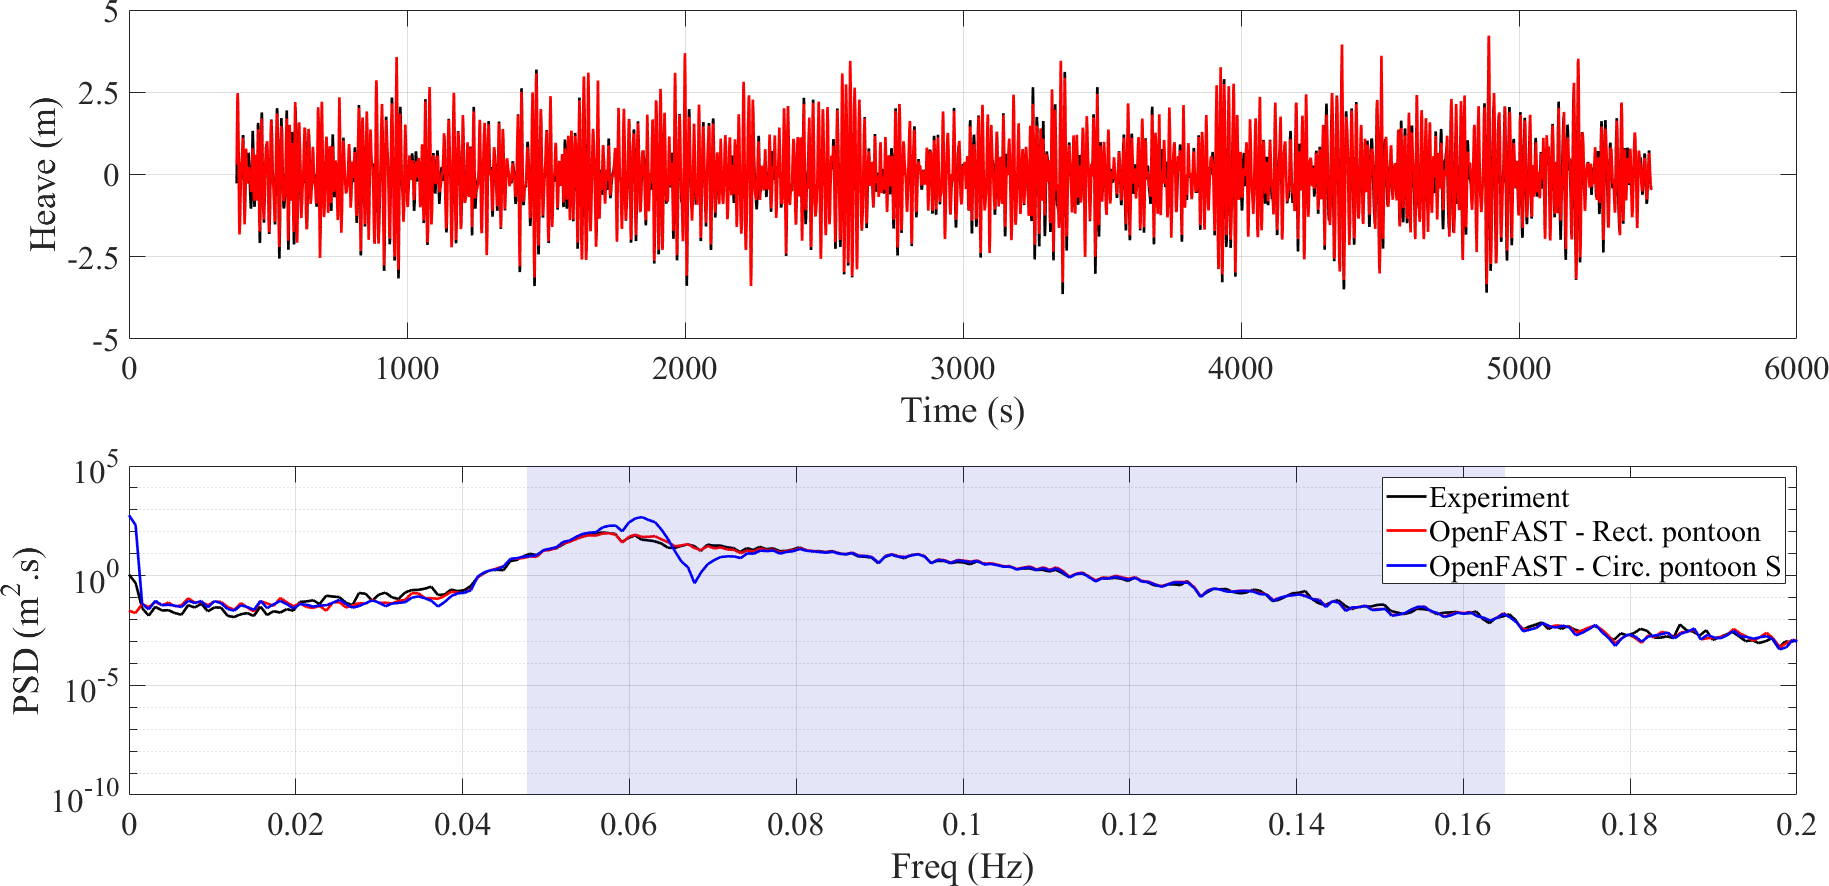
\includegraphics[width=0.9\textwidth]{./figures/ptfmheave-drag_pontoon.png}	
	\caption{Pitch motions obtained with different approaches for the second-order wave forces (IRR-I1 wave, incidence of 60\textdegree{}, without wind effects). The range of frequencies corresponding to the incoming waves is shaded in blue.} \label{fig:exp_vs_num:2ndOrder:ptfmpitch}%
\end{figure*}%









\subsection{The impact of mean hull inclination when computing radiation/diffraction coefficients} \label{subsec:exp_vs_num:impact_inclination}
The third aspect that was investigated is the impact of considering the mean hull inclination caused by the wind when solving the radiation/diffraction problem. For doing so, all the simulations were performed twice: once with radiation/diffraction coefficients calculated considering the inclined meshes described in Section~\ref{sec:numerical_models} (denoted by IC), and once with coefficients computed with an even keel mesh (denoted by EK), as already mentioned in Section~\ref{sec:numerical_models}. The comparisons between these two sets of simulations were based on selected quantities obtained for the \textcolor{red}{220} irregular wave conditions listed in Section~\ref{sec:description_experiment:envir}, namely the motions in the six degrees of freedom, the tensions in the three fairleads, the aerodynamic thrust, and the acceleration at the nacelle (decomposed into an horizontal and a vertical component). 

Since this leads to a large dataset, the different quantities were analyzed by comparing the maximum, mean and standard deviation of each time series. The results are summarized by boxplots of the absolute difference between the values obtained considering the IC and the EK meshes, as presented in Figures~\textcolor{red}{6}, \textcolor{red}{7} and \textcolor{red}{8}. For conciseness, only the maxima are given in this work, but the conclusions are the same for the mean and standard deviation. The graphs show that the differences are very small, specially taking into account that the extra work required to compute individual WAMIT coefficients for each wind condition is very cumbersome and error prone. At least for the test case analyzed in this work, the utilization of a single mesh would allow for a complete set of QTFs to be used instead of the approach of mixing .8 and .9 WAMIT files discussed in Section~\ref{subsec:exp_vs_num:2nd_order}, which has a larger impact than accounting for mesh inclination.

\begin{figure}[!hbtp]
	\centering
	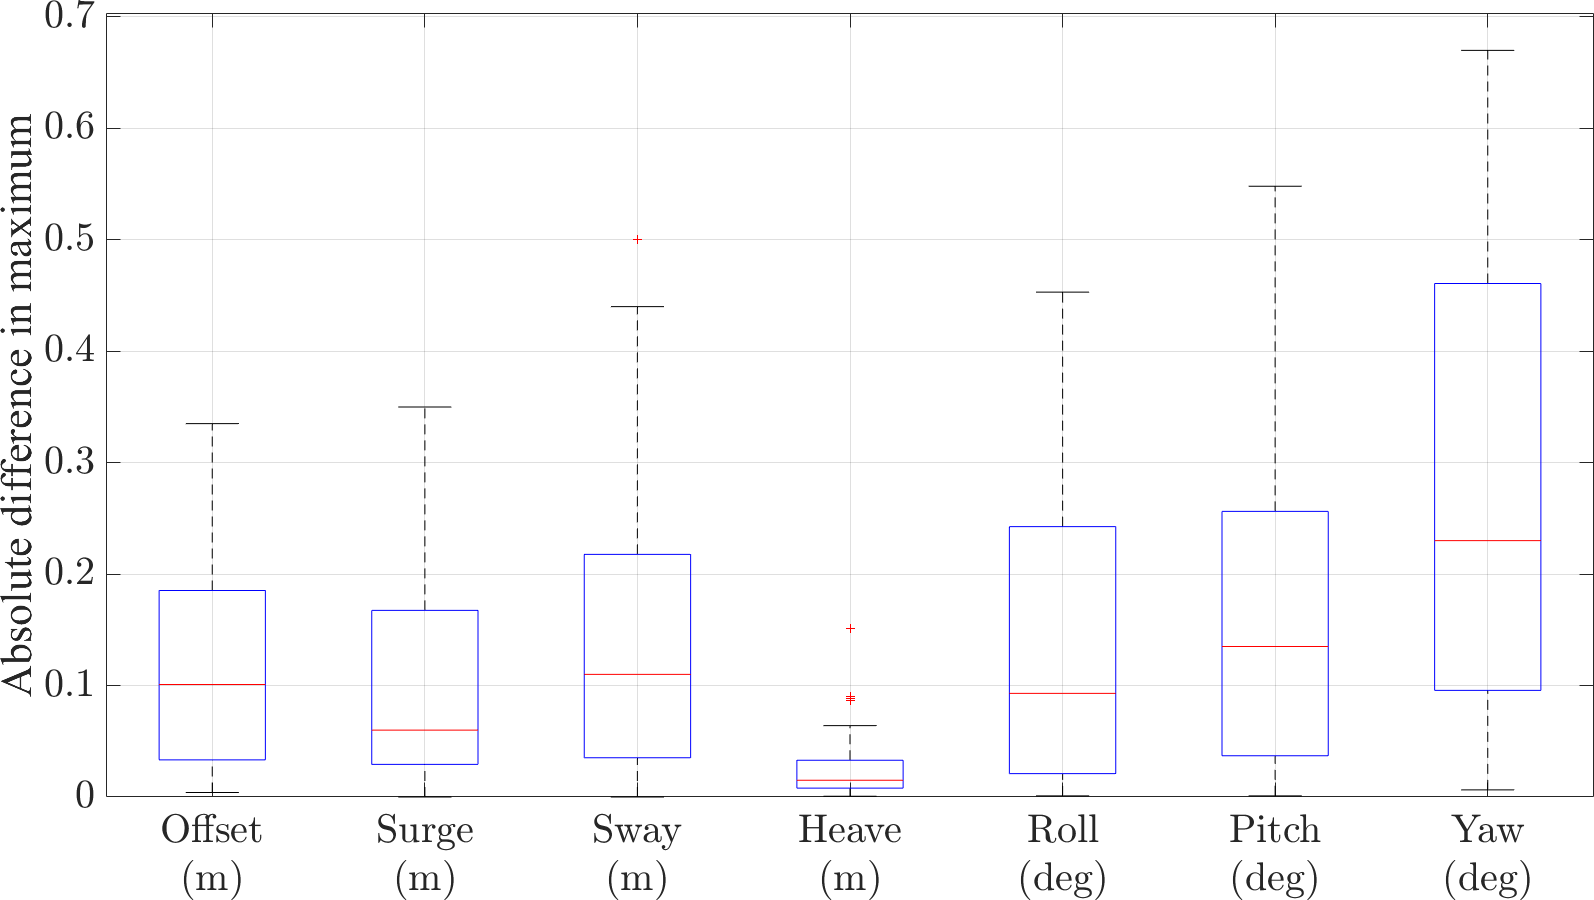
\includegraphics[width=0.5\columnwidth]{./figures/ek_vs_ic-motions}	
	\caption{Pitch motions obtained with different approaches for the second-order wave forces (IRR-I1 wave, incidence of 60\textdegree{}, without wind effects). The range of frequencies corresponding to the incoming waves is shaded in blue.} \label{fig:exp_vs_num:impact_inclination:boxplot-motions}%
\end{figure}%

\begin{figure}[!hbtp]
	\centering
	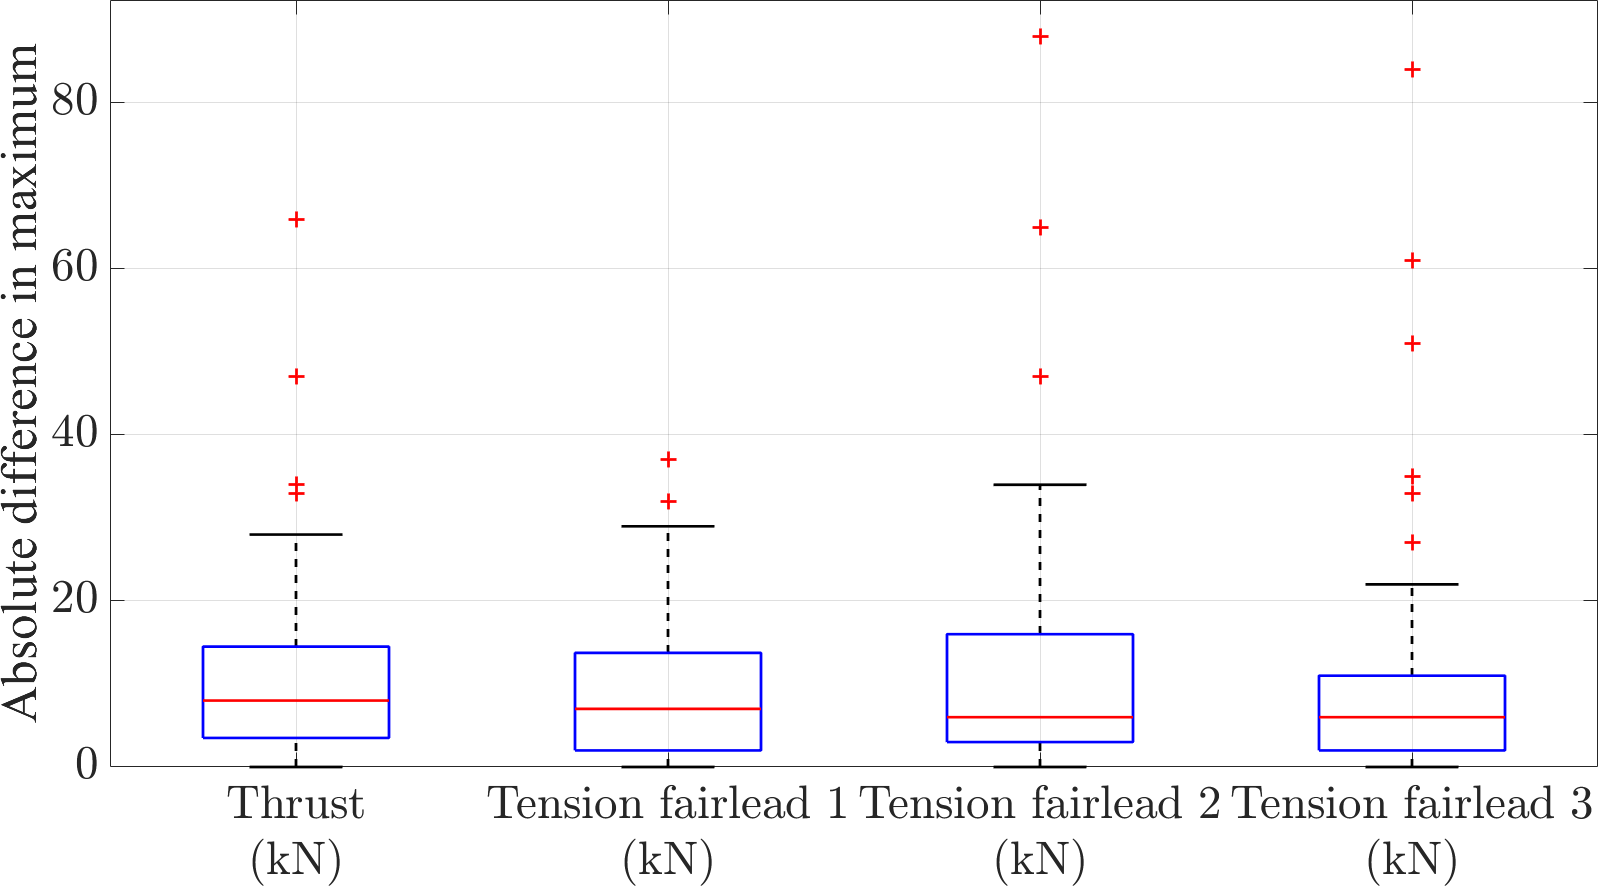
\includegraphics[width=0.5\columnwidth]{./figures/ek_vs_ic-forces}	
	\caption{Pitch motions obtained with different approaches for the second-order wave forces (IRR-I1 wave, incidence of 60\textdegree{}, without wind effects). The range of frequencies corresponding to the incoming waves is shaded in blue.} \label{fig:exp_vs_num:impact_inclination:boxplot-forces}%
\end{figure}%

\begin{figure}[!hbtp]
	\centering
	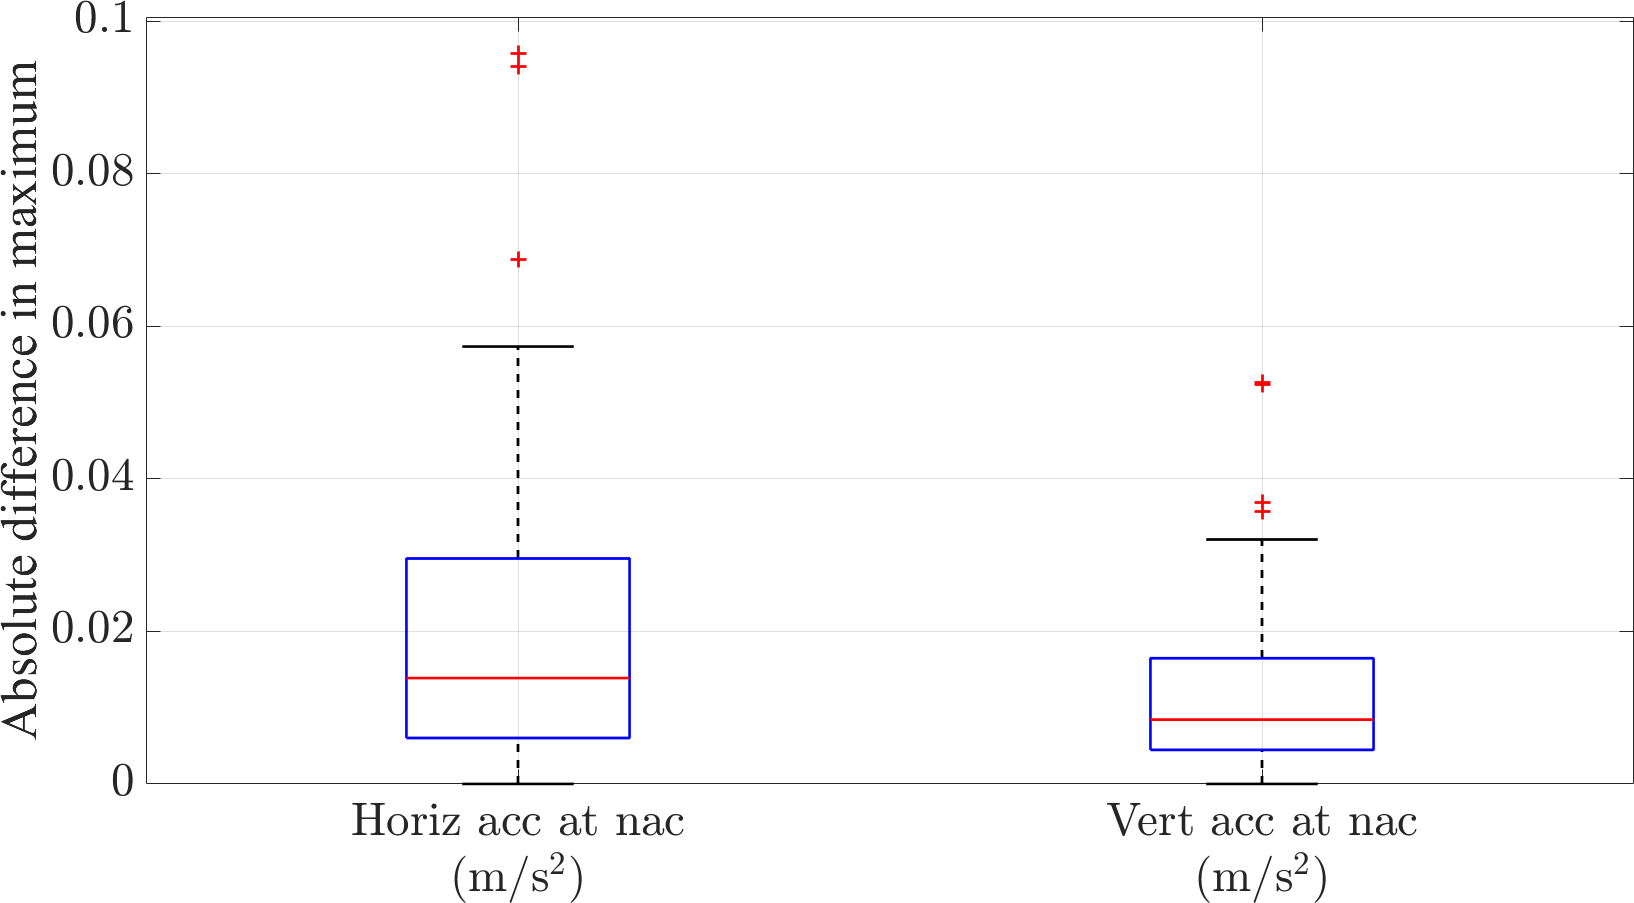
\includegraphics[width=0.5\columnwidth]{./figures/ek_vs_ic-accs}
	\caption{Pitch motions obtained with different approaches for the second-order wave forces (IRR-I1 wave, incidence of 60\textdegree{}, without wind effects). The range of frequencies corresponding to the incoming waves is shaded in blue.} \label{fig:exp_vs_num:impact_inclination:boxplot-accs}%
\end{figure}%

As a more in-depth example, \textcolor{red}{Figure~X} presents the time series and PSDs of roll and pitch motion obtained for the FOWT under the combined action of the IRR12 sea ($H_S=4.44\,\text{m}$, $T_P = 11.34\,\text{s}$ and incidence of -10\textdegree{}) and the turbulent wind condition (mean wind speed $10.59\,\text{s}$ and $\textrm{TI}=12\%$) with an incidence of 47\textdegree{}, which is schematized in the same figure. This case was chosen for being the one that presented the largest difference in the horiontal acceleration at the nacelle, with the IC model considering predicting a maximum horizontal acceleration of $0.85\,\text{m}/\text{s}^2$ and the EK one with providing $0.74\,\text{m}/\text{s}^2$, which is actually closer to the experimental value of $0.64\,\text{m}/\text{s}^2$. 

**Mostrar gráfico de série temporal do que deu a maior diferença**

%In fact, this could be anticipated by looking directly at the radiation/diffraction coefficients that are imported by OpenFAST. These are illustrated by \textcolor{red}{Figure~X} (first-order diffraction forces), \textcolor{red}{Figure~X} (mean drift force) and \textcolor{red}{Figure~X} (added mass and potential damping). For conciseness, only the mesh with the largest inclination (\textcolor{red}{dizer qual é aqui, i.e. p/ qual vento, e qual é a inclinação}) and only one wave incidence (45\textdegree{}) is plotted, and the results for sway and roll are omitted because they are qualitatively the same as surge and pitch.
%
%**Mostrar gráficos das forças**

It is worth pointing out that only the impact of hull inclination on radiation/diffraction coefficients was assessed, and it is possible that it may be important to effects related to real flow phenomena, such as drag forces.





\subsection{Main results} \label{subsec:exp_vs_num:main_results}
Explicar o procedimento adotado para processar a grande quantidade de ondas, que é baseado nas estatísticas.
Mostrar tabela com períodos naturais e níveis de amortecimentos + tabela de resumo das estatísticas p/ ondas irregulares.

Ilustrar c/ gráficos de séries temporais e espectros de casos selecionados (tem que ter a aerodinâmica p/ mostrar que o rotor tá funcionando) + gráfico do máximo e média (tentar colocar um monte na mesma figura)


